%%%%%%%%%%%%%%%%%%%%%%%%%%%%%%%%%%%%%%%%%
% University/School Laboratory Report
% LaTeX Template
% Version 3.1 (25/3/14)
%
% This template has been downloaded from:
% http://www.LaTeXTemplates.com
%
% Original author:
% Linux and Unix Users Group at Virginia Tech Wiki 
% (https://vtluug.org/wiki/Example_LaTeX_chem_lab_report)
%
% License:
% CC BY-NC-SA 3.0 (http://creativecommons.org/licenses/by-nc-sa/3.0/)
%
%%%%%%%%%%%%%%%%%%%%%%%%%%%%%%%%%%%%%%%%%

%----------------------------------------------------------------------------------------
%	PACKAGES AND DOCUMENT CONFIGURATIONS
%----------------------------------------------------------------------------------------

\documentclass{article}

\usepackage[version=3]{mhchem} % Package for chemical equation typesetting
\usepackage{siunitx} % Provides the \SI{}{} and \si{} command for typesetting SI units
\usepackage{graphicx} % Required for the inclusion of images
\usepackage{natbib} % Required to change bibliography style to APA
\usepackage{amsmath} % Required for some math elements 
\usepackage[utf8]{inputenc}
\usepackage[margin=1.3in]{geometry}
\usepackage{hyperref}

\setlength\parindent{0pt} % Removes all indentation from paragraphs

% \renewcommand{\labelenumi}{\alph{enumi}.} % Make numbering in the enumerate environment by letter rather than number (e.g. section 6)

\renewcommand{\figurename}{Figura}
\renewcommand{\tablename}{Tabla}
\renewcommand\refname{Referencias}
\def\mean#1{\left< #1 \right>}
%\usepackage{times} % Uncomment to use the Times New Roman font
\renewcommand{\vec}[1]{\mathbf{#1}}

\usepackage{environ}
\NewEnviron{myequation}{%
\begin{equation}
\scalebox{1.1}{$\BODY$}
\end{equation}
}
%----------------------------------------------------------------------------------------
%	DOCUMENT INFORMATION
%----------------------------------------------------------------------------------------

\title{M\'etodos num\'ericos para la Ciencia e Ingenier\'ia \\ Tarea 11: Ajuste de Curvas Bayesiano} % Title

\author{Felipe Toledo B.} % Author name

\date{\today} % Date for the report

\begin{document}

\maketitle % Insert the title, author and date

%----------------------------------------------------------------------------------------
%	SECTION 1
%----------------------------------------------------------------------------------------

\section{Introducción}

En el presente trabajo se estudian modelos orientados a describir una línea de absorción de una observación espectroscópica, presentada en la Figura \ref{fig:datos_originales}.

\begin{figure}[ht]
  \centering
  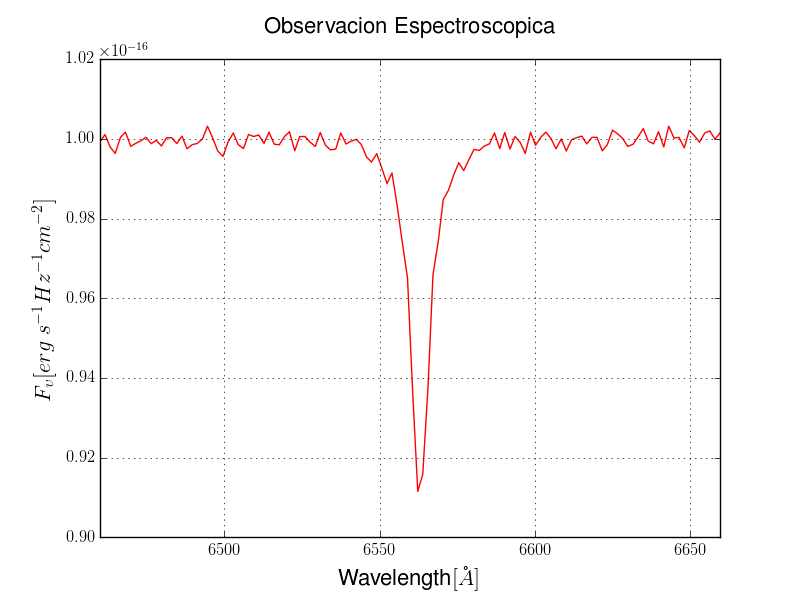
\includegraphics[scale = 0.5]{images/datos_originales.png}
  \caption{Datos originales observados. El nivel del continuo y la longitud de onda central de la línea de absorción son conocidos, con valores $1 \cdot 10^{-16} [\frac{erg}{s\ Hz\ cm^{-2}}]$ y $6563[\AA]$ respectivamente.}
  \label{fig:datos_originales}
\end{figure}

Para describir la línea se probarán dos modelos:

\begin{enumerate}

\item Línea Gaussiana Simple: A partir de la curva se observa que puede resultar conveniente describirla asumiendo que es de forma Gaussiana. En la ecuación (\ref{ec:modelo_1}) se explicita el modelo propuesto. 

\begin{myequation}
M_1(\lambda; A, b) = C_0 - A e^{\frac{-(\lambda - \lambda_0)^2}{2 b^2}}
\label{ec:modelo_1}
\end{myequation}

Éste posee dos parámetros libres, $A$ y $b$. El valor de $\lambda_0$ y $C_0$ se asume conocido, donde $\lambda_0$ es la longitud de onda central de la línea de absorción y $C_0$ corresponde al nivel del continuo.  

\item Línea Gaussiana Doble: El modelo está explicitado en la ecuación (\ref{ec:modelo_2}). Se tienen los mismos parámetros conocidos $\lambda_0$ y $C_0$, pero en éste hay cuatro parámetros libres: $A_1$, $A_2$, $b_1$, $b_2$.

\begin{myequation}
M_2(\lambda; A_1, A_2, b_1, b_2) = C_0 - A_1 e^{\frac{-(\lambda - \lambda_0)^2}{2 b_1^2}} - A_2 e^{\frac{-(\lambda - \lambda_0)^2}{2 b_2^2}}
\label{ec:modelo_2}
\end{myequation}

\end{enumerate}

Los objetivos son: 

\begin{enumerate}
  \item Definir las distribuciones a Priori para cada parámetro.
  
  \item Estimar el valor de los parámetro de cada modelo junto a su intervalo de credibilidad al 68\%, usando métodos Bayesianos.
  
  \item Escoger el modelo que entregue una mejor representación de los datos utilizando técnica Bayesianas.
\end{enumerate}



%%%------------------- METODOLOGIA -----------------------------%%%
\section{Metodología}
\label{sec:metodologia}

Para obtener una estimación de los parámetros $\vec{\Theta}$ para cada modelo $M$, se utiliza la regla de Bayes (\ref{eq:bayes}) y los datos empíricos $\vec{x} = (\vec{\lambda}, \vec{F})$.

\begin{myequation}
  P(\Theta| \vec{x}, M) = \frac{P(\vec{x}|\Theta, M) P(\Theta| M)}{P(\vec{x}|M)}
  \label{eq:bayes}
\end{myequation}

El término $P(\Theta| \vec{x}, M)$ indica la probabilidad a posteriori de que los parámetros representen a los datos $\vec{x}$ para el modelo $M$. Se calcula utilizando la distribución de probabilidad de la derecha, donde $P(\vec{x}|\Theta, M)$ es la verosimilitud, que mide la cercanía de los datos respecto a $M(\Theta)$. La probabilidad $P(\Theta| M)$ corresponde a la distribución a priori de los parámetros, la que se fija arbitrariamente. Finalmente, el término $P(\vec{x}|M)$ es difícil de calcular por lo que se utiliza como constante de normalización, de forma que (\ref{eq:bayes}) queda como (\ref{eq:bayes_2}).

\begin{myequation}
  P(\Theta| \vec{x}, M) = K \cdot P(\vec{x}|\Theta, M) P(\Theta| M)
\label{eq:bayes_2}
\end{myequation} 

Para todos los casos se utiliza la función de verosimilitud (\ref{ec:verosimilitud}), donde $M$ representa el modelo a evaluar. El valor de $\sigma$ corresponde al error asociado a cada punto, el cual se estima usando la desviación estándar de los puntos lejanos a la línea de absorción sobre el continuo ($\approx$ error de medición).

\begin{myequation}
  P(\vec{x}|\Theta, M) = \frac{1}{(2 \pi \sigma^2)^{N/2}} e^{\frac{-1}{2 \sigma^2} \sum\limits_{i=1}^N (F_i - M(\lambda_i, \Theta))^2 }
  \label{ec:verosimilitud}
\end{myequation}

La probabilidad a priori de los parámetros de cada distribución dependerá de cada modelo y se detalla en las secciones \ref{sec:modelo1} y \ref{sec:modelo2}. Con todo lo anterior, se puede calcular $P(\Theta| \vec{x}, M)$, la que permite estimar los valores óptimos\footnote{En este caso se utilizará como valor óptimo $\Theta^*$ al valor $\textbf{E}(\Theta)$ calculado usando $P(\Theta| \vec{x}, M)$.} y sus intervalos de credibilidad.

%%%---------------------- PARAMETROS PARA CADA MODELO ---------------------------%%%
\subsection{Parámetros modelo 1: Línea Gaussiana Simple}
\label{sec:modelo1}

El modelo descrito por (\ref{ec:modelo_1}) posee dos parámetros libres, $A$ y $b$. Para utilizar técnicas Bayesianas de estimación es necesario definir una probabilidad a priori para el valor de cada parámetro. Dado que ambos valores están asociados a datos de un fenómeno continuo (mediciones físicas), serán modelados utilizando funciones Gaussianas.

\subsubsection{Parámetro \emph{A}}

A priori se decide que la distribución de $A$ es:

\begin{myequation}
P(A) = \frac{1}{\sqrt{2 \pi} \sigma_A} e^{\frac{-(A - \bar A)^2}{2 \sigma_{A}^2}}
\label{ec:distr_A}
\end{myequation}

Para determinar el valor de cada parámetro se debe tener en cuenta que A representa la amplitud en Flujo de la curva Gaussiana del modelo. Para determinarlos se presumirá que las mediciones no están muy alejadas de los valores medios esperados. Con todo esto, se decide lo siguiente:

\begin{itemize}
\item $\bar A$ será la amplitud máxima medida respecto al contínuo.

\item $\sigma_A$ corresponderá al error de medición de Flujo. Se utilizará el mismo valor que el $\sigma$ de la verosimilitud, ya que corresponde al mismo fenómeno.
\end{itemize}

\subsubsection{Parámetro \emph{b}}
Análogamente, la distribución escogida para $b$ es:

\begin{myequation}
P(b) = \frac{1}{\sqrt{2 \pi} \sigma_b} e^{\frac{-(b - \bar b)^2}{2 \sigma_{b}^2}}
\end{myequation}

\begin{itemize}
\item $\bar b = 0.8493|\lambda_0 - \lambda(\frac{\bar A}{2})|$

\item $\sigma_b = \Delta$ Se estima a partir de la resolución en longitud de onda (resolución horizontal) del modelo.
\end{itemize}

El valor de $\bar b$ se determina usando la aproximación \emph{Full Width at Half Maximum} (FWHM), donde $\lambda(\frac{\bar A}{2})$ es uno de los valores de longitud de onda en que la línea de absorción cae a la mitad en amplitud\footnote{Se asume que la línea de absorción es aproximadamente simétrica.}.

\subsection{Parámetros modelo 2: Línea Gaussiana Doble}
\label{sec:modelo2}
En este caso la distribución de probabilidad de cada parámetro también será Gaussiana y de forma análoga a los de la Sección \ref{sec:modelo1}. Al determinar los parámetros a Priori se aprovecha la disponibilidad de dos Gaussianas en el modelo, para utilizar una en el ajuste del extremo delgado de la línea y la otra para la base ancha.  Entonces, en resumen:

Para las variables de la curva delgada, $A_1$ y $b_1$:
\begin{itemize}
  \item $\bar{A_1} = \frac{\bar{2A}}{3}$ - La altura media de la línea de absorción debe ser $\approx \bar{A}$ al sumar las exponenciales.
  
  \item $\sigma_{A_1} = \frac{2\sigma_A}{3}$ - El error en $F$ recibe el mismo escalamiento que $A_1$.
  
  \item $\bar{b_1} = \bar{b}$
  
  \item $\sigma_{b_1} = \sigma_b$ - Error asociado al muestreo.
\end{itemize}

Y para la curva ancha, $A_2$ y $b_2$:

\begin{itemize}
  \item $\bar{A_2} = \frac{\bar{A}}{3}$

  \item $\sigma_{A_2} = \frac{\sigma_A}{3}$

  \item $\bar{b_2} = 3\bar{b}$ - Se estima que la base es aproximadamente tres veces mas ancha que la zona delgada.
  
  \item $\sigma_{b_2} = \sigma_b$
\end{itemize}

\section{Selección de Modelo}

Para escoger el modelo más apropiado se comparan sus funciones de verosimilitud (\ref{ec:funcion_verosimilitud}) evaluadas en los datos originales.

\begin{equation}
  P(\vec{x}|M) = \int P(\vec{x}|\Theta, M_i) d\Theta
  \label{ec:funcion_verosimilitud}
\end{equation}

Así, se escogerá como mejor modelo a aquel con el valor de (\ref{ec:funcion_verosimilitud}) más elevado.

\section{Resultados}

Para operar numéricamente con los datos, y evitar \emph{overflows} o divisiones por cero, se escalan los valores del espectro multiplicándolo por $2.5 \cdot 10^{18}$. Esta corrección es considerada e invertida al momento de retornar los valores calculados.

El error de los datos, calculado usando el estimador Gaussiano de varianza\footnote{Se calcula usando los datos con $\lambda < 6525[\AA]$ y $\lambda > 6600[\AA]$. El estimador usado es $\hat{\sigma^2} = \frac{1}{n} \sum\limits_{i=1}^N (F_i - C_0)$.} respecto al continuo, es $\sigma^2 = 0.1695$.

A continuación se presentan en detalle los valores de cada término introducido en la sección Metodología para su modelo correspondiente, junto al ajuste logrado. 

\subsection{Modelo 1: Línea Gaussiana Simple}

Los parámetros estimados a priori son:

\begin{itemize}
  \item $ \bar{A} = 8.848 \cdot 10^{-18} [\frac{erg}{s\ Hz\ cm^{-2}}]$
  
  \item $ \sigma_A = 1.646 \cdot 10^{-19} [\frac{erg}{s\ Hz\ cm^{-2}}]$
  
  \item $ \bar{b} = 4.0 [\AA] $
  
  \item $ \sigma_b = 1.6 [\AA] $
\end{itemize}


Las distribuciones de probabilidad a posteriori para cada estimador pueden observarse en las Figuras \ref{fig:distr_A_modelo1} y \ref{fig:distr_b_modelo1}. A partir de ellas se determinan los valores $\Theta^*$.

\begin{figure}[h!]
  \centering
  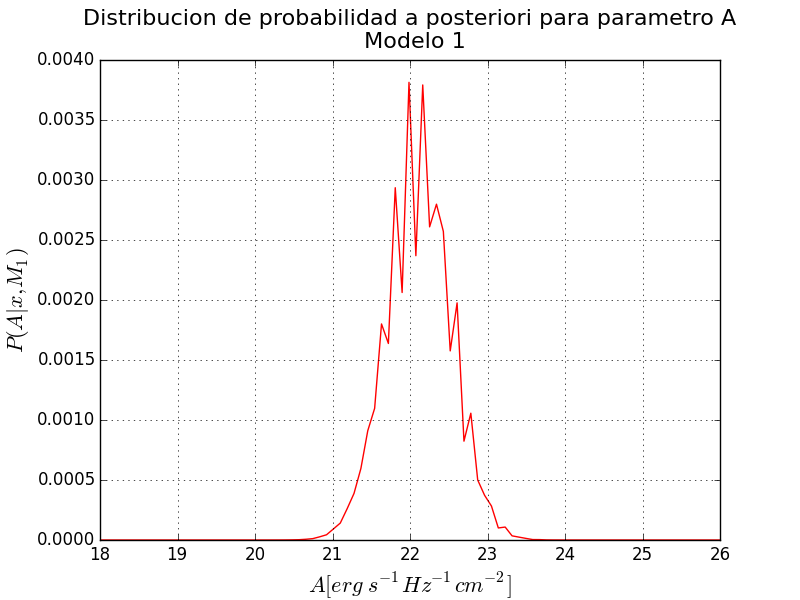
\includegraphics[scale = 0.5]{images/distr_A_modelo1.png}
  \caption{Distribución de probabilidad a posteriori para parámetro A del Modelo 1.}
  \label{fig:distr_A_modelo1}
\end{figure}

\begin{figure}[h!]
  \centering
  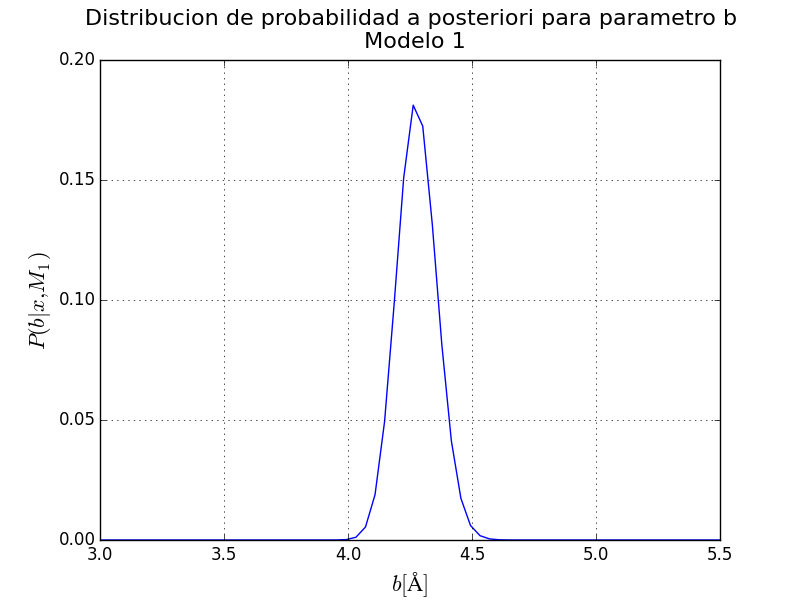
\includegraphics[scale = 0.5]{images/distr_b_modelo1.png}
  \caption{Distribución de probabilidad a posteriori para parámetro b del Modelo 1.}
  \label{fig:distr_b_modelo1}
\end{figure}

Para los intervalos de credibilidad se integra cada distribución desde su valor medio hacia afuera simétricamente, deteniéndose en los valores extremos tales que el valor del área sea 0.68. El enfoque es válido debido a que la distribución a posteriori para cada parámetro está asociada a una densidad de probabilidad.

Así, en resumen, se obtiene:

\begin{itemize}
  \item $A^* = 8.846 \cdot 10^{-18} [\frac{erg}{s\ Hz\ cm^{-2}}]$

  \item Invervalo de credibilidad de $A$ al 68\%: $A \in [8.618,\  9.043] \cdot 10^{-18} [\frac{erg}{s\ Hz\ cm^{-2}}]$

  \item $b^* = 4.2782$
  
  \item Invervalo de credibilidad de $b$ al 68\%: $b \in [4.109,\  4.417] \cdot 10^{-18} [\frac{erg}{s\ Hz\ cm^{-2}}]$
  
\end{itemize}

Con los valores determinados a posteriori para el Modelo 1, se obtiene el ajuste de la Figura \ref{fig:datos_vs_modelo1}.

\clearpage
\begin{figure}[h!]
  \centering
  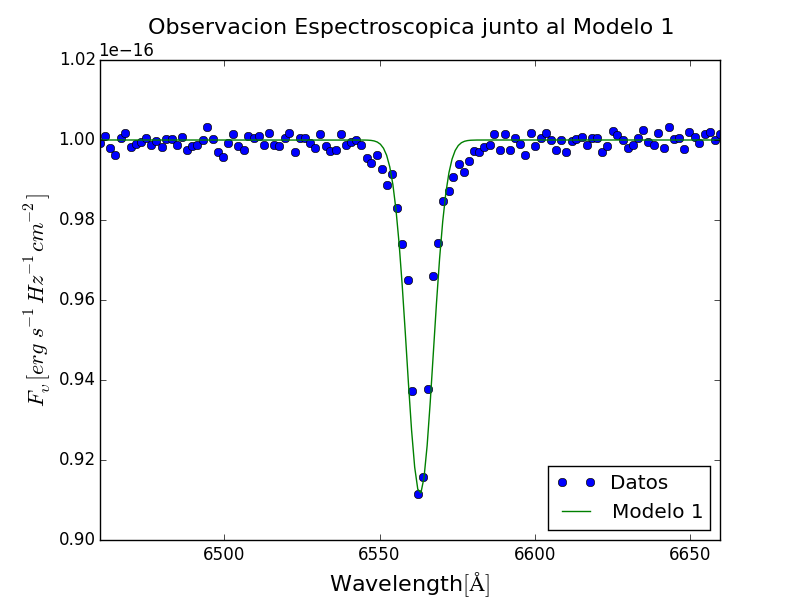
\includegraphics[scale = 0.5]{images/datos_vs_modelo1.png}
  \caption{Ajuste bayesiano del Modelo 1 junto a los datos originales.}
  \label{fig:datos_vs_modelo1}
\end{figure}


\section{Conclusiones}
Se concluye que el método Bayesiano de ajuste de curvas es una buena herramienta para verificar la capacidad que tiene un modelo para describir un fenómeno, mediante la herramienta de funciones de verosimilitud. Esta metodología resulta especialmente atractiva para verificar las capacidades predictivas de modelos teóricos mediante contraste con resultados experimentales. También tiene potenciales aplicaciones en inteligencia artificial. Un sistema inteligente podría inventarse muchos modelos e ir discriminandólos y ajustándolos usando sus observaciones y criterios Bayesianos, de forma que se converja a una \emph{mejor descripción} de su sistema en estudio.

El requerimiento de definir distribuciones a priori para cada parámetro demanda una comprensión, al menos superficial, del fenómeno a describir. Lo mínimo que se necesita conocer es el tipo de distribución. En caso de que no se conozcan los parámetros para alguna variable, se puede lograr un ajuste mediante iteraciones con distintos parámetros en las distribuciones a priori, por ejemplo usando un algoritmo tipo Monte Carlo. Se escogerían entonces aquellos parámetros que maximicen la verosimilitud del modelo. Este tipo de procedimiento queda limitado por la disponibilidad de tiempo de cálculo, que como se sabe puede resultar muy elevado para este tipo de algoritmos. El disponer de mayor información sobre un sistema permite, entonces, obtener tiempos de cálculo más reducidos.

Finalmente, este trabajo ilustra sobre la importancia de implementar métodos de optimización en operaciones matemáticas muy repetitivas. Si se hubiese dispuesto de más series de datos el tiempo de ejecución del programa hubiese aumentado considerablemente debido a la cantidad de integrales que se calculan para obtener el valor de cada parámetro. En caso de dedicarse al trabajo en esta línea, o con algoritmos de monte carlo, se recomienda estudiar técnicas de optimización de código tanto a nivel de algoritmos como conscientes de la arquitectura del procesador (por ejemplo utilizar \emph{multithreading)}, ya que tanto esta experiencia como las anteriores indican que el tiempo de cómputo es una limitante crucial.


\end{document}
